\documentclass[%
        %draft,
        %submission,
        %compressed,
        final,
        %
        %technote,
        %internal,
        %submitted,
        %inpress,
        %reprint,
        %
        %titlepage,
        notitlepage,
        %anonymous,
        narroweqnarray,
        inline,
        %twoside,
        ]{ieee}
%
% some standard modes are:
%
% \documentclass[draft,narroweqnarray,inline]{ieee}
% \documentclass[submission,anonymous,narroweqnarray,inline]{ieee}
% \documentclass[final,narroweqnarray,inline]{ieee}

% Use the `endfloat' package to move figures and tables to the end
% of the paper. Useful for `submission' mode.
%\usepackage {endfloat}

% Use the `times' package to use Helvetica and Times-Roman fonts
% instead of the standard Computer Modern fonts. Useful for the 
% IEEE Computer Society transactions.
% (Note: If you have the commercial package `mathtime,' it is much
% better, but the `times' package works too).
%\usepackage {times}

% In order to use the figure-defining commands in ieeefig.sty...
\usepackage{ieeefig}
\usepackage{pdflscape}
\usepackage{rotating}
\usepackage{graphicx}
\usepackage{multirow}
\usepackage{dcolumn}
\usepackage{booktabs}

\begin{document}

%----------------------------------------------------------------------
% Title Information, Abstract and Keywords
%----------------------------------------------------------------------
\title[18.353 Final Project]{The Interaction Dynamics of Bay Scallops, Cownose Rays, and Hammerhead Sharks}

% format author this way for journal articles.
\author[John Wang]{}

% specifiy the journal name
\journal{18.353 Final Project}

% Or, when the paper is a preprint, try this...
%\journal{IEEE Transactions on Something, 1997, TN\#9999.}

% Or, specify the conference place and date.
\confplacedate{Ottawa, Canada, May 19--21, 1997}

% make the title
\maketitle               

% do the abstract
\abstract{The preservation of natural ecosystems has become an increasingly important area of research. In this paper, we examine the dynamics of the hammerhead shark (\textit{Sphyrna lewini}), cownose ray (\textit{Rhinoptera bonasus}), and bay scallop (\textit{Argopecten irradians}) populations. We examine how shark to ray and ray to scallop predation can affect the entire ecosystem. We estimate parameters of the system for the east coast of the United States and analyze the impact of fishing.}


\section{Introduction}

We consider the following ecosystem, where $X,Y,$ and $Z$ are the number of scallops, cownose rays, and hammerhead sharks respectively. We assume these populations evolve continuously as:
\begin{eqnarray}
\dot{X} &=& R_0 X(1 - X/K_0) - C_1 F_1(X) Y \nonumber \\
\dot{Y} &=& F_1 (X) Y - F_2 (Y) Z - D_1 Y \\
\dot{Z} &=& C_2 F_2(Y) Z - D_2 Z \nonumber \\
\mathrm{where} \hspace{0.5cm} F_i(U) &=& \frac{A_i U}{B_i + U} \nonumber
\end{eqnarray}

We can nondimensionalize the system using the following dimensionless variables:
\begin{eqnarray}
x &=& X/K_0 \nonumber \\
y &=& C_1 Y/ K_0 \nonumber \\
z &=& C_1 Z / (C_2 K_0) \\
t &=& R_0 T \nonumber
\end{eqnarray}

Which leads to the following nondimensionalized system:
\begin{eqnarray}
\dot{x} &=& x(1-x) - f_1(x) y \nonumber \\
\dot{y} &=& f_1(x) y - f_2(y) z - d_1 y \\
\dot{z} &=& f_2(y) z - d_2 z \nonumber \\
\mathrm{where} \hspace{0.5cm} f_i(u) &=& \frac{a_i u}{1 + b_i u} \nonumber
\end{eqnarray}

\section{Parameter Interpretations}

It is evident that $K_0$ represents the carrying capacity of the scallops, and $R_0$ represents the logistic growth rate of the population. The conversion factors $C_1$ and $C_2$ must have dimensions [scallops/rays] and [sharks/rays] in order for them to nondimensionalize $y$ and $z$. These parameters represent the carrying capacity of rays and sharks in terms of $K_0$. One can also see that $D_1$ is the death rate of a rays and $D_2$ is the death rate of sharks. 

Analyzing the functions $F_i$ show that they must have dimensions of [1/time]. This means that $A_i$ has units of [1/time] and $B_i$ has units of population. $A_i$ represents the frequency of predation in a unit of time, while $B_i$ represents a close to average population size. 

\section{Parameter Values}

In light of these observations, we can attempt to fit these parameter values to our problem. First, we will only consider the region where scallops and cownose rays are prominent, which is on the eastern coast of the United States. We will pick the area where scallops usually inhabit, which roughly corresponds to the coastline between North Carolina and Cape Cod. This is about 800 miles of coastline, and scallops inhabit up to about 3 miles offshore \cite{Fay(1983)}. Scallop densities in the late 1970s and early 1980s were about 20 scallops per square meter, which is historically close to the highest density reached \cite{Fay(1983)}. This means that we have a carrying capacity of roughly $K_0 = 1 \times 10^{11}$ scallops in our region. The average density of scallops now has dropped dramatically and is probably closer to 5 scallops per square meter, which leads to roughly $B_1 = 2 \times 10^{10}$. 

Next, we note that cownose rays consume about 1.5\% of their body weight each day according to \cite{Neer(2005)} who determines consumption based on $VO_2$ respiration. The average cownose ray weighs about 10kg while the average scallop weighs about 0.02kg. Thus, assuming scallops consist for about 50% of a ray's diet, the average ray consumes about 1300 scallops per year. If we assume that cownose rays eat scallops five times a day, we have parameter values of roughly $A_1 = 5$ and $C_1 =380$. 

The average density of cownose rays in Chesepeake Bay is roughly 0.001 rays per square meter \cite{Blaylock(1993)}. We can estimate $C_1$ from this data as well. Assuming we have roughly a density of 2.5 scallops per square meter (since scallop densities dropped off dramatically since \cite{Fay(1983)} performed their measurements), we see that there are about $C_1 = 2.5/(0.001*5) = 500$ scallops per ray. Taking the average of the two $C_1$ values we obtained, we will use $C_1 =  440$. We can also obtain the parameter for the average population of rays $B_2 = 5 \times 10^{6}$ using this estimate.

Hammerhead sharks consume about 2\% of their body weight each day \cite{Bush(2002)}. Since hammerheads weigh about 150kg, and cownose rays are about 10kg, we see that hammerheads consume about 50 cownose rays per year if we assume cownose rays account for about 50\% of the hammerhead diet. Thus, we find the parameter values of $A_2 = 3$ and $ C_2 = 1/50 = 0.02$.  

Death rates can be obtained by looking at average lifetimes and assuming uniform distributions of age. Cownose rays live for about 15 years, so we obtain $D_1 = 0.07$, while hammerheads live about 25 years, so $D_2 = 0.04$. We assume a growth rate of $R_0 = 20$. 

%\begin{table}[ht!]
%\centering
%\caption{\sffamily{Parameter Value Estimates}}
%\setlength{\extrarowheight}{2pt}
%\begin{tabular}{@{}>{\sffamily}l >{\sffamily}l >{\sffamily}l >{\sffamily}c >{\sffamily}c} 
%\toprule[1.5pt]
% & Paremeter & Dimension & Estimated Value & References \\
%\midrule
%\multicolumn{5}{l}{\textbf{Dimensionless Conversion Parameters}} \\
%&$C_1$ & [scallops/rays] & 440 & \cite{Neer(2005)} and \cite{Blaylock(1993)}\\
%&$C_2$ & [sharks/rays] & 0.02 & \cite{Bush(2002)}\\
%\\[-8pt]
%\multicolumn{5}{l}{\textbf{$F_1$ and $F_2$ Function Parameters}} \\
%&$A_1$ & [1/time] & 5 & \\
%&$A_2$ & [rays/(time $*$ sharks)] & 3 & \\
%&$B_1$ & [scallops] & $2 \times 10^{10}$ & \cite{Fay(1983)} \\
%&$B_2$ & [rays] & $5 \times 10^{6}$ & \cite{Blaylock(1993)} \\
%\\[-8pt]
%\multicolumn{5}{l}{\textbf{Scallop Population Parameters}} \\
%&$K_0$ & [scallops] & $1 \times 10^{11}$ & \cite{Fay(1983)} \\
%&$R_0$ & [1/time] & 20 & \\
%\\[-8pt]
%\multicolumn{5}{l}{\textbf{Death Rates}} \\
%&$D_1$ & [1/time] & 0.07 & \\
%&$D_2$ & [1/time] & 0.04 & \\
%\bottomrule[1.5pt]
%\end{tabular}
%\end{table}

\section{Dimensionless Parameters}

Since we have estimates for the parameters in our original equations, we can find the nondimensionalized parameters. We can express the nondimensionalized equations in terms of the dimensionalized coefficients and find:
\begin{eqnarray}
\frac{dx}{dt} &=& \frac{dX}{dT} \frac{1}{K_0 R_0} = \frac{1}{K_0 R_0} \left( R_0 X \left(1 - \frac{X}{K_0} \right) - C_1 \frac{A_1 X}{B_1 + X} Y \right) \nonumber \\
&=& x(1-x) - \frac{\frac{A_1 K_0}{R_0 B_1} x}{1 + \frac{K_0}{B_1} x} y \\
\frac{dy}{dt} &=& \frac{dY}{dT} \frac{C_1}{R_0 K_0} = \frac{C_1}{R_0 K_0} \left( \frac{A_1 X}{B_1 + X} Y - \frac{A_2 Y}{B_2 + Y} Z - D_1 Y \right) \nonumber \\
&=& \frac{ \frac{A_1 K_0}{R_0 B_1} x}{1 + \frac{K_0}{B_1} x} y - \frac{\frac{A_2 K_0 C_2}{R_0 B_2 C_1}y}{1 + \frac{K_0}{B_2 C_1} y } z - \frac{D_1}{R_0} y \\
\frac{dz}{dt} &=& \frac{dZ}{dT} \frac{C_1}{R_0 C_2 K_0} = \frac{C_1}{R_0 C_2 K_0} \left( C_2 \frac{A_2 Y}{B_2 + Y} Z - D_2 Z \right) \nonumber \\
&=& \frac{ \frac{C_2 A_2 K_0}{R_0 B_2 C_1} y}{1 + \frac{ K_0}{B_2 C_1} y} z - \frac{D_2}{R_0} z  
\end{eqnarray}

Using these equations, we can obtain the expressions for the dimensionless parameters in terms of the parameters from the original equation. Using these expressions, we can obtain estimated values for $a_i, b_i$, and $d_i$ based on the estimated values for the parameters from the original equation. Substituting these values into the dimensionless equations, we have:
\begin{eqnarray}
\dot{x} &=& x(1-x) - \frac{x }{1 + 5 x}y \\
\dot{y} &=& \frac{x}{1 + 5 x} y - \frac{0.1 y}{1 + 45 y} z - d_1 y \\
\dot{z} &=& \frac{0.1 y}{1 + 45 y} z - d_2 z
\end{eqnarray}

%\begin{table}[ht!]
%\centering
%\caption{\sffamily{Dimensionless Parameters}}
%\setlength{\extrarowheight}{2pt}
%\begin{tabular}{@{}>{\sffamily}l >{\sffamily}l >{\sffamily}l >{\sffamily}r } 
%\toprule[1.5pt]
% & Parameter & Expression & Estimated Value  \\
%\midrule
%\multicolumn{4}{l}{\textbf{$F_1$ and $F_2$ Function Parameters}} \\
%&$a_1$ & $\frac{A_1 K_0}{R_0 B_1}$ & 1 \\
%&$a_2$ & $\frac{A_2 K_0 C_2}{R_0 B_2 C_1}$ & 0.1 \\
%&$b_1$ & $\frac{K_0}{B_1}$ & 5  \\
%&$b_2$ & $\frac{K_0}{B_2 C_1}$ & 45\\
%\\[-8pt]
%\multicolumn{4}{l}{\textbf{Death Rates}} \\
%&$d_1$ & $\frac{D_1}{R_0}$ & $4 \times 10^{-3}$ \\
%&$d_2$ & $\frac{D_2}{R_0}$ & $2 \times 10^{-3}$ \\
%\bottomrule[1.5pt]
%\end{tabular}
%\end{table}

\section{Fixed Points}

The first analysis one can perform is to look for fixed points of the nondimensionalized system where $\frac{d}{dt}\vec{x} = 0$. A trivial fixed point is where $\vec{x}_1 = (0,0,0)$. To analyze its local stability, we can linearize and find the Jacobian of the system evaluated at $\vec{x}_1$. The Jacobian is:
\begin{equation}
J = \left[ \begin{array}{ c c c}
1 - 2x - \frac{a_1 y}{(1 + b_1 x)^2} & - \frac{a_1 x }{1 + b_1 x} & 0 \\
\frac{a_1 y}{(1 + b_1 x)^2} & \frac{a_1 x}{1 + b_1 x} - \frac{a_2 z}{(1 + b_2 y)^2} - d1 & - \frac{a_2 y}{1 + b_2 y} \\
0 & \frac{a_2 z}{(1 + b_2 y)^2} & \frac{a_2 y}{1 + b_2 y} - d_2 
\end{array} \right]
\end{equation}

Substituting $(x,y,z) = (0,0,0)$ into the Jacobian, we find:
\begin{equation}
J(0,0,0) = \left[ \begin{array}{c c c}
1 & 0 & 0 \\
0 & -d1 & 0 \\
0 & 0 & - d2
\end{array} \right]
\end{equation}

It is clear that the linearized equations decouple and we obtain $x(t) = x_0 e^t, y(t) = y_0 e^{-d_1 t},$ and $ z(t) = z_0 e^{-d_1 t}$. Since $d_1$ and $d_2$ are death rates which are always positive, we see that $y(t)$ and $z(t)$ decay to 0. However, the $x(t)$ equation grows with time. Physically, this means that small perturbations about the origin lead to the ray and shark populations to dying out, while the scallop populations will increase and be repelled from the origin. This makes intuitive sense because small populations of all three animals means the predators will most likely die off, while the scallop population without predators should increase. 

The other fixed point that occurs for all parameters is $\vec{x}_2 = (1,0,0)$. The Jacobian at $\vec{x}_2$ is the following:
\begin{equation}
J(1,0,0)J = \left[ \begin{array}{ c c c}
-1 & -\frac{a_1}{1 + b_1} & 0 \\
0 & \frac{a_1}{1 + b_1} - d_1 & 0 \\
0 & 0 & -d_2 
\end{array} \right]
\end{equation}

Notice that the Jacobian is upper triangular so that the eigenvalues lie on the diagonals. The fixed point is locally stable if all the eigenvalues are negative, which is equivalent to the condition that $a_1/(1 + b_1) < d_1$.  Also notice that the equations decouple, since one can solve explicitly for $z(t) = z_0 e^{-d_2 t}$ and $y(t) = y_0 e^{(a_1/(1 + b_1) - d_1) t}$. Using our parameter estimates, we find $a_1 / (1 + b_1) = 0.17 \not < 4 \times 10^{-3}$. Thus, the $\vec{x}_2$ fixed point in our regime is not locally stable. 

\section{Limit Cycles and Attractors}

Numerical experiments suggest that there exists an attractor somewhere in the region about the origin, but only in the $xy$ plane. We will show analytically that this attracting region exists as long as $d_1 < a_1 / (1 + b_1)$. Notice that this is the same condition for the $\vec{x}_2 = (1,0,0)$ fixed point to be unstable. After the analysis, it will be clear that the local stability of the $\vec{x}_2$ fixed point will be governed by the appearance of the attracting region, so that the appearance of the limit cycle will correspond exactly with the change in stability of $\vec{x}_2$. 

We see the trajectory in figure \ref{attractor} has periodic oscillations in the $xy$ plane. It seems to be bounded by some boxed region about the origin. Let us define this region in $xy$ space as $[0,x_h] \times [0, y_h]$, where $x_h$ and $y_h$ are constant values of $x$ and $y$ respectively. Clearly, trajectories can't leave the region through the $x$ or $y$ axis because $x,y \geq 0$ by the physical limitations of the system, and because once $x=0$ ($y = 0$) then $x$ stays 0 forever (similarly with $y = 0$). Therefore, we need to make sure no trajectories leave from the vertical $x = x_h$ line and the horizontal $y = y_h$ line. 

On the vertical $x = x_h$ line, we need to check that $\dot{x} < 0$, so that trajectories only enter the region. We have:
\begin{equation}
\dot{x} = x_h(1 - x_h) - \frac{a_1 x_h}{1 + b_1 x_h} y
\end{equation}

The second term in this equation is always negative. The largest it can be is $0$ when $y = 0$. Thus, $x_h ( 1 - x_h) < 0$ is a sufficient condition for $\dot{x} < 0$. This implies that $x_h > 1$ will guarantee that trajectories only enter the region through the $x = x_h$ vertical line. 

On the horizontal line $y = y_h$, we need to check that $\dot{y} < 0$:
\begin{equation}
\dot{y} = \frac{a_1 x}{1 + b_1 x} y_h - \frac{a_2 y_h}{1 + b_2 y_h} z - d_1 y_h
\end{equation}

Clearly the second and third terms are always nonpositive. The second term's maximum occurs when $z = 0$. The coefficient of the first term $a_1 x / (1 + b_1 x)$ is an increasing function in $x$. We know that the maximum value of $x$ in the region is $x_h > 1$. Thus, the maximum value of the first term is $a_1 / (1 + b_1)$, and occurs when $x_h = 1$. Therefore, we see that $\dot{y} < 0$ exactly when:
\begin{equation}
\frac{a_1}{1 + b_1} > d_1
\end{equation}

Thus, there exists a trapping region $[0,x_h] \times [0, y_h]$ when $a_1 / (1 + b_1) > d_1$ (since the first condition $x_h > 1$ can always be satisfied). 

\subsection{Attractor Existence}
\label{sec:attractorexist}

Notice that there is a fixed point that might exist inside the trapping region. This occurs at 
\begin{equation}
\vec{x}_3 = (x^{*},y^{*},z^{*}) = \left( \frac{d_1}{a_1 - b_1 d_1}, \frac{a_1 - d_1 - b_1 d_1}{(a_1 - b_1 d_1)^2}, 0 \right)
\end{equation}

The $a_1 / (1 + b1) > d_1$ condition guarantees that $a_1 > d_1 (1 + b_1)$ so that $y^{*} > 0$ when the trapping region exists, since the numerator $a_1 - d_1(1 + b_1) >0$ and the denominator $(a_1 - b_1 d_1)^2$ is always positive. Since we can choose any $y_h$ line for which $\dot{y} < 0$ given our condition of $a_1 > d_1 ( 1 + b_1)$, we can choose $y_h > y^{*}$. This means that the $y$ coordinate of $\vec{x}_3$ is inside the trapping region, so that $0 < y^{*} < y_h$.

To show that the $x^{*}$ coordinate must be inside the trapping region, we must have $a_1 > b_1 d_1$ for $x^{*} > 0$. This follows directly from the $a_1 - d_1(1 + b_1) > 0$ condition, since $a_1 - b_1 d_1 > d_1$ and $d_1 \geq 0$, so that $a_1 - b_1 d_1 > 0$. Moreover, since $a_1 - b_1 d_1 > d_1$, we see that $x^{*} = d_1 / (a_1 - b_1 d_1) < 1 = x_h$. Therefore $0 < x^{*} < x_h$, which means the $x$ coordinate of $\vec{x}_3$ must lie in the trapping region if it exists. Thus if the trapping region exists, then the fixed point $\vec{x}_3$ will always exist in the trapping region. 

It is difficult to analytically examine stability of $\vec{x}_3$, since the Jacobian evaluated at $\vec{x}_3$ gives a complicated expression. However, we can make qualitative observations. If $\vec{x}_3$ is unstable and we have parameters such that no other fixed point exists in the trapping region, then there must be some type of attracting manifold. This follows because all trajectories flow into the trapping region, but never settle down to any fixed point. 

\subsection{Example System with Attracting Manifold}

Using certain parameters, we can show there exists some attracting manifold inside the $xy$ trapping region. Take $b_1 = 5, b_2 = 45, a_2 = 0.1, d_2 = 0.002$ like before, but now change $d_1 = 2$ and $a_1 = 25$. This corresponds to a regime where fishing of rays increases dramatically. Our analysis has shown that a trapping region should exist when $a_1 / (1 + b_1) > d_1$, which is indeed the case since $a_1 ( 1 + b_1) = 25 / 6 > d_1 = 2$. Moreover, one can numerically solve for the Jacobian at $\vec{x}_3 = (0.13, 0.06, 0)$. The eigenvalues of the linearized system are $0.11 \pm 1.0i$ and $-4.0 \times 10^{-4}$. The real parts of the complex eigenvalues are positive and shows that the fixed point at $\vec{x}_3$ is unstable. Moreover, one can numerically show that the other fixed points with real, nonnegative values are $\vec{x}_1 = (0,0,0)$ and  $\vec{x}_2 = (1,0,0)$. Thus, $\vec{x}_3$ is the only fixed point that lies inside the trapping region. Since it is unstable, our analysis in section \ref{sec:attractorexist} shows that we should see an attracting manifold.

Indeed, this is the case. Figure \ref{attractor} shows a trajectory entering the trapping region given these parameters. Changing the $d_1$ parameter to $a_1 ( 1 + b_1) + 0.01$ eliminates the manifold, as seen in figure \ref{noattractor}, although one can see a ghost of the cylindrical shape in the trajectories.

\figdef{attractor}

%\begin{figure}[h!]
%\centering
%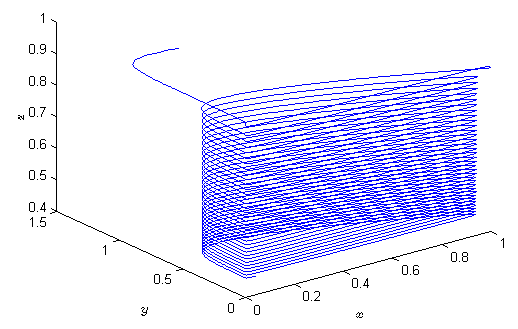
\includegraphics[width=2.5in]{attractor.png}
%\caption{Cylindrical Attractor}
%\label{attractor}
%\end{figure}
%
%\begin{figure}[h!]
%\centering
%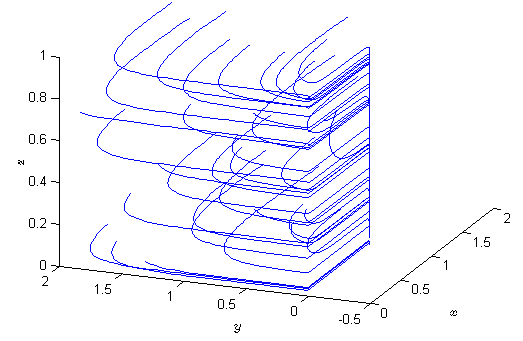
\includegraphics[width=2.5in]{noattractor.png}
%\caption{Ghost of Cylindrical Attractor}
%\label{noattractor}
%\end{figure}

\bibliographystyle{IEEEbib}
\bibliography{bibliography}
\nocite{*}

\end{document}
